\section{Implementierung}
Mit der Implementierung wird bei dem Mechanismus zur Auswahl gestartet.

% Fragen
Wie wird der jeweilige Punkt umgesetzt?

Welche Tools werden benutzt/eignen sich besonders für die Umsetzung?
Welche Tools eignen sich für welchen Arbeitsschritt?

Warum wird etwas gerade auf diese Weise umgesetzt?



Umsetzen des jeweiligen Architekturpunktes:
Wie Factory, 
Hardwareauswahl
Objekterstellung
Wie Peripherals: GPIO, SPI
Objekterstellung
Funktionsimplementierung

Unterscheiden zwischen ESP32 und STM32

Projektstruktur
make
Makefile
config.mk

CMake Struktur
CMakeLists
\\
1. Struktur aufsetzen\\
- man weiss was man braucht\\
- ein Rootverzeichnis HW\_API, enthält alles: Treiber, Peripherie Module, Anleitung, CMake-Struktur, Makefile\\
- als erstes die CMake-Struktur aufsetzen.\\
- dazu wird der Verzeichnisbaum  grundlegend erstellt.\\
- Verzeichnisse, die enthalten sein müssen, jedes mit eigenem CMakeLists.txt:\\
-- app: enthält main.cpp und main.hpp\\
-- HW\_API: API Root Verzeichnis\\
-- HW\_API/core: enthält Dateien, die allgemein bzw. für mehr als eine Hardware gültig sind. 
	Hier befindet sich die hw\_factory die die Hardware-Objekte erstellt, indem sie die richtigen Treiber anhand von definierten Makros auswählt; C++ Äquivalent zu C Strukturen: enum class, die Hardware-spezifische Makros zusammenfassen; das allgemeine Hardwareinterface, von dem alle unterstützte Hardware erbt.\\
-- HW\_API/debug\_probes: enthält Hilfsdateien zum debuggen. Diese Dateien rufen im Hintergrund die entsprechenden Programme auf, die für die gewünschte Debug-Art bzw. für die verwendete Hardware notwendig sind.\\
-- HW\_API/drivers/stm32\_hal\_wrapper bzw. /esp32\_hal\_wrapper: enthalten Hardware-spezifische Konfigurationsdateien für die jeweiligen Mikrocontroller-Plattformen, die als Brücke (Wrapper) zwischen der herstellerspezifischen Hardware-Abstraktionsschicht (HAL) und der plattformunabhängigen HW\_API dienen.
	Die enthaltenen Konfigurationsdateien definieren Makros über:\\
	--> Hardwareressourcen: Speichergröße, Peripherie-Ausstattung, Taktfrequenzen\\
	--> Peripherie-Aktivierung: Welche Hardware-Module (GPIO, SPI, I2C, UART, etc.) aktiviert sind\\
	--> Feature-Flags: Welche spezifischen Funktionen der jeweiligen HAL verwendet werden\\
	--> Interrupt-Prioritäten: Konfiguration des NVIC (Nested Vectored Interrupt Controller)\\
	--> Low-Level-Initialisierung: Hardware-spezifische Initialisierungssequenzen\\
	Die Wrapper-Schicht ermöglicht es der HW\_API, mit einer einheitlichen Schnittstelle auf unterschiedliche Hardware zuzugreifen, während die plattformspezifischen Details vor den höheren Schichten verborgen bleiben. Dies ist ein wesentlicher Bestandteil der Hardware-Abstraktion und ermöglicht die Portierbarkeit der Anwendung zwischen verschiedenen Mikrocontroller-Familien.
	Die Konfigurationsdateien werden beim Build-Prozess automatisch eingebunden und bestimmen das Verhalten der Hardware-Abstraktionsschicht auf der jeweiligen Zielplattform.\\
-- HW\_API/platform: Dieses Verzeichnis bildet das Herzstück der Hardwareabstraktion und enthält die plattformspezifischen Implementierungen der Hardware-API. \\
	Es ist nach folgendem Konzept strukturiert:\\
	--> Plattform-Trennung: Separierte Unterordner für jede unterstützte Hardwareplattform (stm32, esp32)\\
	--> Familie-Spezialisierung: Weitere Unterteilung nach Mikrocontroller-Familien (stm32c0, stm32f4, esp32s3)\\
	--> Interface-Implementierung: Konkrete Implementierungen der in den Core-Modulen definierten abstrakten Interfaces\\
	Schlüsselkomponenten:\\
	--> Hardware-Treiber: Implementieren die konkreten Hardware-Zugriffsfunktionen\\
	--> Register-Abstraktion: Kapseln direkten Register-Zugriff in typsichere C++-Interfaces\\
	--> Hardware-Mapping: Übersetzen zwischen logischen Ressourcen und physischen Hardware-Adressen\\
	--> Interrupt-Handler: Plattformspezifische Interrupt-Implementierungen\\
	--> Clock-Konfiguration: MCU-spezifische Takteinstellungen und Power-Management\\
	Die Plattform-Schicht nutzt die HAL-Wrapper (aus dem drivers-Verzeichnis) und bietet nach oben eine einheitliche Schnittstelle für die Core-Module. \\
	Dies ermöglicht es, dass der Rest der Applikation hardwareunabhängig bleibt, während diese Schicht die tatsächlichen Unterschiede zwischen den Mikrocontroller-Plattformen abstrahiert.\\
	Ein wesentliches Designprinzip ist, dass alle hardwarespezifischen Details innerhalb dieser Schicht gekapselt bleiben und nicht in höhere Schichten durchsickern.\\
-- HW\_API/peripherie Modul (gpio, spi, can, ...): Diese Verzeichnisse enthalten die Peripherie-spezifischen Module der Hardware-Abstraktionsschicht für GPIO (General Purpose Input/Output) und SPI (Serial Peripheral Interface). \\
	Sie bilden die Brücke zwischen den generischen Hardware-Interfaces und den konkreten Implementierungen für verschiedene Plattformen.\\
	Struktur und Komponenten:\\
	--> Interface-Definitionen: Abstrakte Basisklassen und Interfaces, die die Funktionalität der jeweiligen Peripherie definieren\\
	--> Gemeinsame Datentypen: Enums, Strukturen und Konstanten, die die Konfigurationsparameter der Peripherie repräsentieren\\
	--> Plattformunabhängige Logik: Gemeinsamer Code, der für alle Plattformen gleich funktioniert\\
	--> Factory-Klassen: Erzeugen plattformspezifische Implementierungen basierend auf Konfigurationsparametern\\
	Typische Dateien im GPIO-Modul:\\
	--> gpio\_interface.hpp: Definiert die abstrakte GPIO-Schnittstelle\\
	--> gpio\_types.hpp: Gemeinsame Datentypen wie PinMode, PullType, etc.\\
	Typische Dateien im SPI-Modul:\\
	--> spi\_interface.hpp: Definiert die abstrakte SPI-Schnittstelle\\
	--> spi\_types.hpp: Datentypen für SPI-Konfigurationen (Mode, Geschwindigkeit, Bit-Reihenfolge)\\
	Diese Module arbeiten eng mit dem Platform-Layer zusammen, der die tatsächlichen Hardware-spezifischen Implementierungen enthält.\\ Die Anwendung interagiert nur mit den abstrakten Interfaces, während die konkreten Implementierungen zur Kompilierzeit basierend auf der Zielplattform ausgewählt werden.\\
	Die Peripherie-Module sind so konzipiert, dass sie einfach erweiterbar sind und neue Hardware-Plattformen mit minimalen Änderungen integriert werden können, indem lediglich plattformspezifische Implementierungen hinzugefügt werden, ohne die öffentlichen Schnittstellen zu ändern.\\
-- toolchains: enthält .cmake-Dateien, die die Hardwarespezifischen Compiler \\
	Dieses Verzeichnis enthält die CMake-Toolchain-Dateien, die für die Cross-Compilation auf verschiedene Zielplattformen essentiell sind.\\
	Sie definieren die grundlegenden Compiler-Werkzeuge und Einstellungen, die CMake verwenden soll, um Code für die jeweiligen Mikrocontroller zu kompilieren.\\
	Wichtige Toolchain-Dateien:\\
	--> stm32-toolchain.cmake: Konfiguriert den ARM-GCC-Toolchain für STM32-Mikrocontroller\\
	--> esp32-toolchain.cmake: Konfiguriert den Xtensa-ESP32-Toolchain für ESP32-Mikrocontroller\\
	Diese Dateien definieren:
	--> Compiler-Pfade: Lokalisierung der plattformspezifischen Cross-Compiler (arm-none-eabi-gcc, xtensa-esp32-elf-gcc)\\
	--> Basis-Compiler-Flags: MCU-spezifische Optionen wie CPU-Typ, FPU-Einstellungen und ABI\\
	--> Optimierungs-Einstellungen: Debug- und Release-Konfigurationen mit entsprechenden Optimierungsstufen\\
	--> Linker-Einstellungen: Memory-Sections, Garbage Collection und spezielle Embedded-Linker-Flags\\
	--> Hilfswerkzeuge: Konfiguration von objcopy, objdump und size für Binary-Manipulation\\
	--> Build-Typen: Definitionen für Debug, Release und andere Build-Konfigurationen\\
	Die Toolchain-Dateien werden beim CMake-Aufruf durch den -DCMAKE\_TOOLCHAIN\_FILE-Parameter eingebunden und stellen sicher, dass der gesamte Build-Prozess mit den korrekten Werkzeugen und Einstellungen für die Zielplattform durchgeführt wird.\\
	Sie sind ein kritischer Bestandteil des Cross-Compilation-Workflows und ermöglichen die Entwicklung auf einem Host-System für eine andere Zielarchitektur.\\
	Diese Konfigurationsdateien werden vom Makefile-System automatisch ausgewählt, basierend auf der gewählten Zielplattform, sodass Entwickler nicht manuell zwischen verschiedenen Toolchains wechseln müssen.

2. Implementierung:\\







\vspace{5mm}

% Oszi-Bild , wie es aussehen sollte
\begin{figure}[H]
	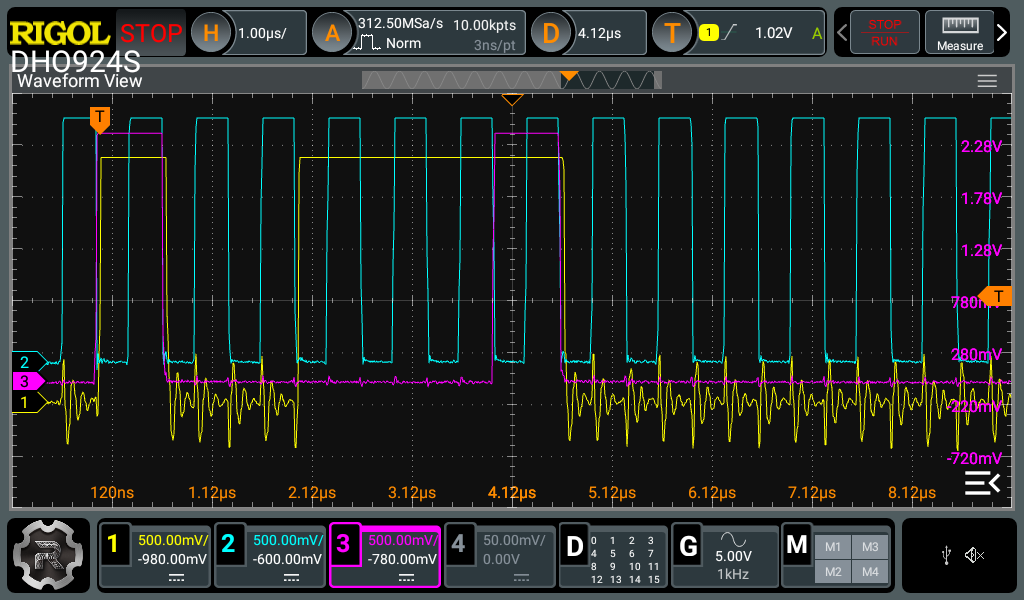
\includegraphics[width=\textwidth]{Pics/oszi_cube_spi_example.png}
	\caption{Screenshot des Osziloskopbildschirms. Dieser zeigt die Wellen für SCK (blau), MOSI (magenta) und MISO (gelb).}
	\label{fig:oszi_cube_spi_example}
\end{figure}

So sollten die Wellen auch mit dem Plattformunabhängigen Code aussehen.














































